\documentclass[10pt, a4paper]{article}
\usepackage[utf8]{inputenc}
\usepackage[T1]{fontenc,url}
\usepackage{multicol}
\usepackage{multirow}
\usepackage{parskip}
\usepackage{lmodern}
\usepackage{microtype}
\usepackage{verbatim}
\usepackage{amsmath, amssymb}
\usepackage{tikz}
\usepackage{physics}
\usepackage{mathtools}
\usepackage{algorithm}
\usepackage{algpseudocode}
\usepackage{listings}
\usepackage{enumerate}
\usepackage{graphicx}
\usepackage{float}
\usepackage{hyperref}
\usepackage{tabularx}
\usepackage{siunitx}
\usepackage{fancyvrb}
%\usepackage{natbib}
%\bibliographystyle{dinat}
\usepackage[makeroom]{cancel}
\usepackage[margin=2.0cm]{geometry}
\usepackage{pdfpages}
\usepackage[margin=10pt, textfont={small, it}, labelfont={bf}, labelsep=endash]{caption}
\renewcommand{\baselinestretch}{1}
\renewcommand{\exp}{e^}
\renewcommand{\b}{\boldsymbol}
\newcommand{\h}{\hat}
\newcommand{\m}{\mathbb}
\newcommand{\half}{\frac{1}{2}}
\renewcommand{\exp}{e^}
\renewcommand{\bar}{\overline}
\setlength\parindent{0pt}


\begin{document}
\title{AST5220\\ Milestone IV -- Pertubations}
\author{
    \begin{tabular}{r l}
        Jonas Gahr Sturtzel Lunde & (\texttt{jonassl})
    \end{tabular}}
% \date{}    % if commented out, the date is set to the current date

\maketitle
Code found at \url{https://github.com/asdfbat/AST5220/tree/master/Project}
\vspace{0.7cm}

\section{Introduction}


\section{Theory and method}
\subsection{The source function}
Traditionally, the CMB power spectrum was solved for by solving the coupled Boltzmann ODE for all $\ell$'s, which usually ran in the thousands. Due to a clever trick called line-of-sight integration, we need only to calculate the first handful of $\Theta_\ell$s with the full Boltzmann treatment, which we did in the previous milestone, and generate the rest from the so-called \textit{source function}.

The source function is shown in equation \ref{eqn:source}. It consists of four terms, each of which contributes an effect on photons, either \textit{at} last scattering, or as the photons travels from last scattering and towards us.

\begin{equation}
    \label{eqn:source}
    \tilde{S}(k, x) = 
    \underbrace{\tilde{g}\left[\Theta_{0}+\Psi+\frac{1}{4} \Pi\right]}_{SW}
    + \underbrace{e^{-\tau}\left[\Psi^{\prime}-\Phi^{\prime}\right]}_{ISW}
    - \underbrace{\frac{1}{c k} \frac{d}{d x}\left(\mathcal{H} \tilde{g} v_{b}\right)}_{Doppler}
    + \underbrace{\frac{3}{4 c^{2} k^{2}} \frac{d}{d x}\left[\mathcal{H} \frac{d}{d x}(\mathcal{H} \tilde{g} \Pi)\right]}_{Quadrupole}
\end{equation}



\subsection{The multipoles}
With the source function at hand, calculating the photon temperature multipoles is rather trivial, and takes the form of the integral

\begin{equation}
    \Theta_{\ell}(k, x=0)=\int_{-\infty}^{0} \tilde{S}(k, x) j_{\ell}\left(k\left(\eta_{0}-\eta\right)\right) \dd{x}
\end{equation}
where $j_\ell(x)$ is the $\ell$'th Bessel function.


\subsection{Matter power spectrum}
Another quantity of interest which can be calculated from information at hand, even though not related to the photon temperature, is the matter power spectrum, which traces the (linear) perturbations of matter in the universe.

\begin{equation}
    P(k, x) = P_{\text {p}}(k) \Delta_{M}(k, x)^{2}
\end{equation}

where $\Delta_M$ is the (gauge invariant) matter perturbations, defined as
\begin{equation}
    \Delta_{M}(k, x) \equiv \frac{c^{2} k^{2} \Phi(k, x)}{\frac{3}{2} \Omega_{M 0} a^{-1} H_{0}^{2}}
\end{equation}
and $P_\text{p}(k)$ is the \textit{primordial} power spectrum, which is the power spectrum set up by the initial perturbations in the early universe, which is
\begin{equation}
    P_\text{p}(k) = A_s k^{n_s-1}
\end{equation}



\section{Implementation}


\section{Results}
\subsection{Matter power spectrum}
Figure \ref{fig:MatterPower} shows the calculated matter power spectrum, with the point of $k_{peak}$ marked. We clearly see the primordial power spectrum slope of $\propto k^{n_s} \approx k$ before the peak, and the suppressed high k end with slope of $\propto k^{n_s-4} \approx k^{-3}$. The reason for the suppression on the high k end of the spectrum is the Meszaros effect, where small perturbations which entered the horizon before transitioning to the matter dominated era are suppressed by a power of $k^4$.

\begin{figure}[h!]
    \centering
    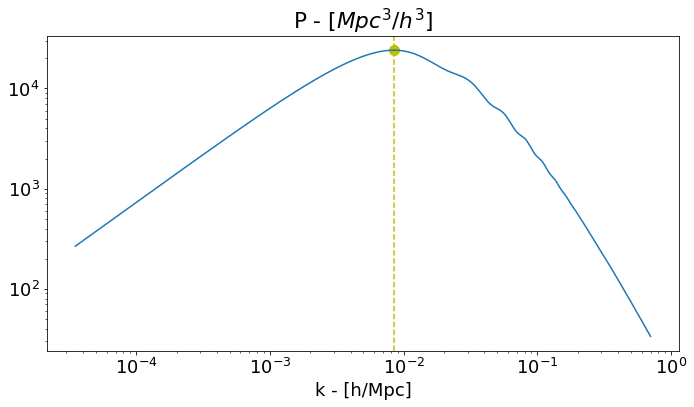
\includegraphics[scale=0.5]{../m4_figs/MatterPower.png}
    \caption{Matter power spectrum in $Mpc^3/h^3$. The "turnover point", corresponding to the peak of the spectrum, is marked at $k=\SI{0.012}{Mpc} = \SI{0.0084}{Mpc/h}$.}
    \label{fig:MatterPower}
\end{figure}


\begin{figure}[h!]
    \centering
    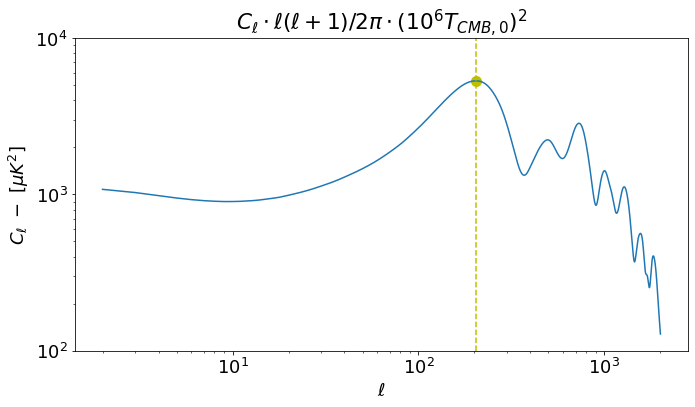
\includegraphics[scale=0.5]{../m4_figs/Cell.png}
    \caption{}
    \label{}
\end{figure}

\begin{figure}[h!]
    \centering
    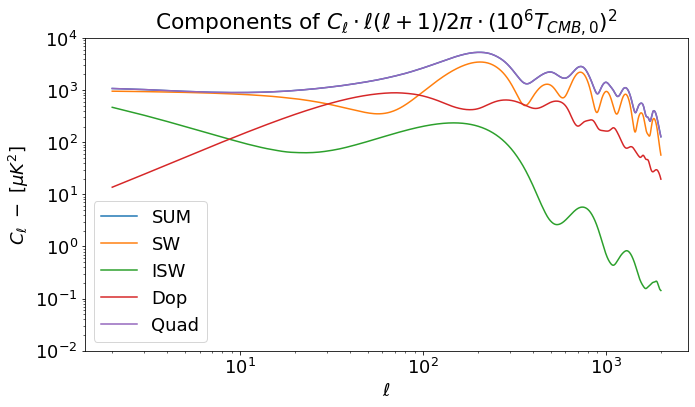
\includegraphics[scale=0.5]{../m4_figs/Cell_all.png}
    \caption{}
    \label{}
\end{figure}


\begin{figure}[h!]
    \centering
    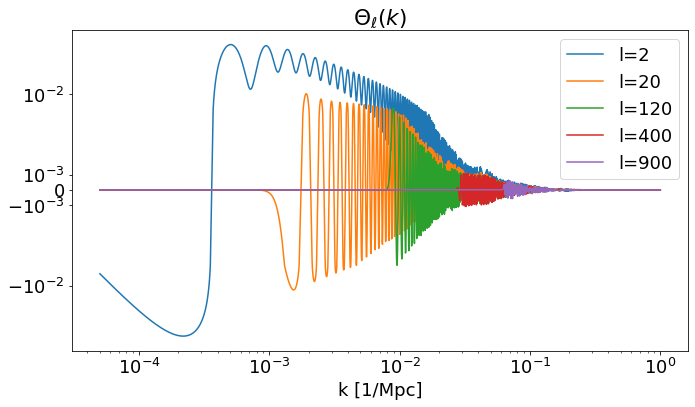
\includegraphics[scale=0.5]{../m4_figs/Theta.png}
    \caption{}
    \label{}
\end{figure}

\begin{figure}[h!]
    \centering
    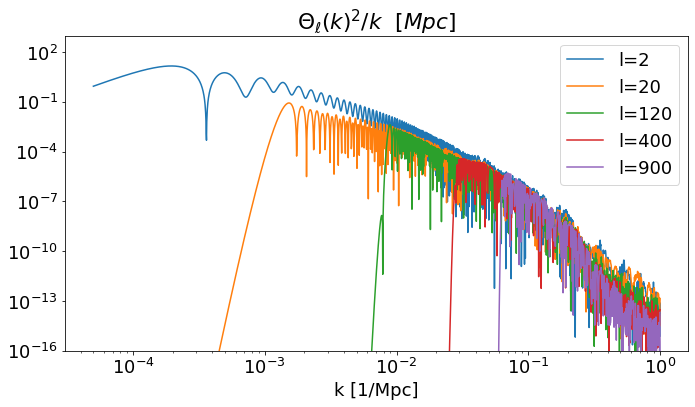
\includegraphics[scale=0.5]{../m4_figs/Theta2.png}
    \caption{}
    \label{}
\end{figure}



\newpage
\bibliography{ref}
\bibliographystyle{plain}



\end{document}